\ifx \allfiles \undefined		%编译PPT时注释该行
	\documentclass{book}
		%%%%%%%%%%%%%%%%%%%%%%%%%%%%%%%%%%%%%%%%%
% 模板資訊:
% 模板名稱:Beamer
% 版本:1.0 (2023.07.09)
% 修改者:Ernie
% 編譯器:XeLaTeX
%
% 原始模板的資訊:
% 模板名稱:Beamer Presentation
% 作者:Vel (vel@latextemplates.com)
% 編譯器:XeLaTeX
% 授權:CC BY-NC-SA 4.0 (https://creativecommons.org/licenses/by-nc-sa/4.0/)
% 下載連結:https://www.LaTeXTemplates.com
%
% 製作本模板之目的:
% 為了讓 LaTeX 初學者能夠輕鬆地完成專業的學術簡報,因此我針對 Vel 製作的模板做了大幅度的修改及附上清楚明瞭的註解。
%
% 如果您有任何問題,可以透過 Email 聯繫我們:stateconlab@gmail.com
% 
% p.s. 也別忘了關注我們的 YouTube、IG 和 Medium 喔!
% 1. YouTube:https://www.youtube.com/@StatEconLab
% 2. IG:https://www.instagram.com/stateconlab
% 3. Mediun:https://medium.com/@stateconlab
%%%%%%%%%%%%%%%%%%%%%%%%%%%%%%%%%%%%%%%%%

%----------------------------------------------------------------------------------------
%	封包與文檔配置
%----------------------------------------------------------------------------------------

\usepackage[space,noindent]{ctex}

% 自訂字體顏色的封包
\usepackage{xcolor} 

%% 自訂顏色

\definecolor{pbblue}{HTML}{0A75A8}% color for the progress bar and the circle
% 數學工具及符號
%\usepackage{mathtools, amsmath, amsfonts, amsthm, latexsym} 

% 分別將數學符號間的間隔加大及加粗
%\usepackage{newtxtext,newtxmath}

% 圖表自動編號的封包
%\usepackage{caption} 

%% 設定自動編號
%\setbeamertemplate{caption}[numbered]

%% 設定圖表編號及標籤的字體大小及字形
%\captionsetup[figure]{font=small, labelfont=md}
%\captionsetup[table]{font=small, labelfont=md}

% 導入圖形與表格的封包
%\usepackage{graphicx}  % \scalebox{} 可用於將過大的表格縮小
%\usepackage{booktabs}

% 排列多個子圖形的封包
%\usepackage{subfigure} 

% 允許表格的一格能多列呈現的封包
%\usepackage{multirow} 

% 可指定表格排版的封包
%\usepackage{array}

% 翻轉表格的封包
%\usepackage{lscape} 

% 序列標號
%\usepackage{enumerate} 

% 繪圖封包 (用於添加浮水印)
\usepackage{tikz}

% 引注參考資料
%\usepackage{natbib}

% 註釋掉大部分的封包
%\usepackage{comment}

\usetikzlibrary{shapes,fit,calc,positioning}

% 設定中文的標籤
%\renewcommand{\figurename}{圖} 
\renewcommand{\tablename}{表} 

%----------------------------------------------------------------------------------------
%	排版形式 (擇一,不選等同選擇默認的排版形式)
%----------------------------------------------------------------------------------------

%\mode<presentation>{
%\usetheme{default}
%\usetheme{AnnArbor}
%\usetheme{Antibes}
%\usetheme{Bergen}
%\usetheme{Berkeley}%演示主题为侧边导航条
%\usetheme{Berlin}
\usetheme{Boadilla}%蓝色主题
%\usetheme{CambridgeUS}
%\usetheme{Copenhagen}
%\usetheme{Darmstadt}
%\usetheme{Dresden}
%\usetheme{Frankfurt}
%\usetheme{Goettingen}
%\usetheme{Hannover}
%\usetheme{Ilmenau}
%\usetheme{JuanLesPins}
%\usetheme{Luebeck}
%\usetheme{Madrid}
%\usetheme{Malmoe}
%\usetheme{Marburg}
%\usetheme{Montpellier}
%\usetheme{PaloAlto}
%\usetheme{Pittsburgh}
%\usetheme{Rochester}
%\usetheme{Singapore}
%\usetheme{Szeged}
%\usetheme{Warsaw}

%----------------------------------------------------------------------------------------
%	外框形式 (擇一,不選等同選擇默認的外框形式)
%----------------------------------------------------------------------------------------

%\useoutertheme{default}
%\useoutertheme{infolines}
%\useoutertheme{miniframes}
%\useoutertheme{smoothbars}
%\useoutertheme{sidebar}
%\useoutertheme{split}
%\useoutertheme{shadow}
%\useoutertheme{tree}
%\useoutertheme{smoothtree}

%----------------------------------------------------------------------------------------
%	外框的自訂義調整 
%----------------------------------------------------------------------------------------

% 外框上緣的字 (fg) 為黑色,背景 (bg) 為白色。
%\setbeamercolor{section in head/foot}{fg=white, bg=black} 

% 外框上緣顯示的章節(section)頁數標籤是否關閉
%\setbeamertemplate{mini frames}{}   

% 調整外框形式的字體大小
%\setbeamerfont{headline}{size=\scriptsize}
%\setbeamerfont{footline}{size=\scriptsize}

% 取消右下方的跳轉工具列
\setbeamertemplate{navigation symbols}{} 

%% 自定義1:外框下緣僅出現名字及頁碼
%\setbeamertemplate{footline}
%{\leavevmode%
%\hbox{%
%\begin{beamercolorbox}[wd=0.5\paperwidth,ht=3ex,dp=1ex,leftskip=2ex]%
%{author in head/foot}%
%{\footnotesize\textbf{\insertshortauthor}}%
%\end{beamercolorbox}%
%\begin{beamercolorbox}[wd=0.5\paperwidth,ht=3ex,dp=1ex,right]%
%{author in head/foot}%
%\footnotesize \textbf{{\insertframenumber{} / \inserttotalframenumber\hspace*{2ex}}} %頁碼控制選項
%\end{beamercolorbox}%
%}}

%% 自定義2:清除外框下緣但僅出頁碼
%\setbeamertemplate{footline}[page number] 

%% 自定義3:清除外框下緣
%\setbeamertemplate{footline}[] 

%----------------------------------------------------------------------------------------
%	顏色主題 (擇一,不選等同選擇默認的顏色主題)
%----------------------------------------------------------------------------------------

%\usecolortheme{default}
%\usecolortheme{albatross}
%\usecolortheme{beaver}
%\usecolortheme{beetle}
%\usecolortheme{crane}
%\usecolortheme{dolphin}
%\usecolortheme{dove}
%\usecolortheme{fly}
%\usecolortheme{lily}
%\usecolortheme{orchid}
%\usecolortheme{rose}
%\usecolortheme{seagull}
%\usecolortheme{seahorse}
\usecolortheme{whale}%颜色主题为
%\usecolortheme{wolverine}

%----------------------------------------------------------------------------------------
%	顏色主題的自訂義調整 
%----------------------------------------------------------------------------------------

% 全文的主題色 (可以特別針對報告對象或機構的代表色調整!)
%\setbeamercolor{structure}{fg=Myblue} 

% 封面頁中標題區塊的底色及字體顏色
%\setbeamercolor{title}{bg=green, fg=black} 

% 各頁標題區塊的底色及字體顏色
%\setbeamercolor{frametitle}{bg=white,fg=black} 

% 全文的內文顏色
%\setbeamercolor{normal text}{fg=orange}

% 數學區塊的標題顏色 
%\setbeamercolor{block title}{bg=blue,fg=yellow} 

% 數學區塊的內文顏色 
%\setbeamercolor{block body}{bg=green,fg=red} 

% 警示文字的顏色
%\setbeamercolor{alerted text}{fg=red} 

%----------------------------------------------------------------------------------------
%	enumerate 及 item 的形狀
%----------------------------------------------------------------------------------------

%\useinnertheme{rounded} % 圓球 (3D)
%\useinnertheme{circles} % 圓形 (2D)
%\useinnertheme{rectangles} % 方形
%\useinnertheme{triangle} % 三角形
%\useinnertheme{inmargin} % 插入邊沿
%\setbeamertemplate{itemize items}[triangle]

%----------------------------------------------------------------------------------------
%	自訂 item 的顏色
%----------------------------------------------------------------------------------------

%\setbeamercolor{item projected}{bg=red}

%----------------------------------------------------------------------------------------
%	個人化的設置及細節調整
%----------------------------------------------------------------------------------------

% 設定頁面邊界
%\setbeamersize{text margin left=0.6cm, text margin right=0.6cm}
%\special{papersize=\the\paperwidth,\the\paperheight}
%\providecommand{\tabularnewline}{\\}
%}

%----------------------------------------------------------------------------------------
%	個人化的背景調控
%----------------------------------------------------------------------------------------

% 背景照片設置
%\setbeamertemplate{background}{\includegraphics[height=\paperheight]{Fig/Background.png}}

% 浮水印設定
%\usebackgroundtemplate{%
%	\tikz[overlay, remember picture] % 讓 logo 能每頁都顯示
%	\node[opacity=0.3, below=-1.25cm, at=(current page.center)] % 調整透明度 (opacity) 及浮水印的位置
%	{\includegraphics[scale = 0.14]{Fig/nthulogo.png}}; % 載入 logo 及調整大小
%	}

		\begin{document}
\else						%编译PPT时注释该行
	%\newpage
\fi						%编译PPT时注释该行
		\watermark{50}{9}{热工班组}
		\chapter[2024年02月份技术培训考试]{	\hspace*{-0.3em}\biaoti{2024}{02}{热工专业}}
		姓名:\uline{ \ \  \  \ \ \ \ \ \ \ \ \ \ \ \ \ \ }\hfill 得分:\uline{ \ \  \  \ \ \ \ \ \  \ \ \ \ \ \ }
		\section{\xzt{5}{2}{10}}
			\begin{enumerate}
				\item 我厂氨水缓冲装置控制系统正常运行过程中,下列哪一个环节退出运行不会影响系统运行\xz{A}。
					\xx{控制器组态软件}{OPC通讯软件}{winCC监控软件}{SMART PLC}
				\item 我厂1、2、3号汽轮机DEH系统Triview监控软件数据中断时需要检查并重启以下哪个程序\xz{B}。
					\xx{Triview监控软件}{DDE通讯软件}{TriStation组态软件}{Diagnostic诊断软件}
				\item 我厂1、2、3号汽轮机DEH系统硬件故障时应该使用以下哪个程序进行检查诊断\xz{D}。
					\xx{SOE记录查询软件}{DDE通讯软件}{TriStation组态软件}{Diagnostic诊断软件}
				\item S7 SMART PLC控制器与上位机通讯使用以下那种通讯方式\xz{A}
					\xx{OPC通讯}{RS 232/485通讯}{CAN通讯}{PROFIBUS通讯}
				\item  S7 200 PLC控制器与上位机通讯使用以下那种通讯方式\xz{B}
					\xx{OPC通讯}{RS 232/485通讯}{CAN通讯}{PROFIBUS通讯}
			\end{enumerate}
		\section{\tkt{4}{2}{30}}
			\begin{enumerate}
				\setcounter{enumi}{5}
				\item 我厂脱硝CEMS系统PLC型号为CPU 224 CN AC/DC/RLY,其中AC/DC/RLY分别对应着\tk{电源电压}/\tk{输入电压}/\tk{输出电压},AC表示交流\tk{220V},DC表示\tk{直流24V},RLY表示\tk{继电器输出}。
				\item PLC有五种标准编程语言:\tk{梯形图语言}、指令表语言(IL)、\tk{功能模块语言}、顺序功能流程图语言(SFC)、结构文本化语言(ST)。对于有电路基础的人来说,\tk{梯形图}是最容易学习的,因为它与电气操作原理图相对应,具有直观性和对应性;与原有继电器控制相一致,电气设计人员易于掌握。
				\item 模拟量信号是自动化过程控制系统中最基本的过程信号,系统中的过程信号通过变送器,将这些检测信号转换为标准的电压、电流信号,常见的标准信号有0-5V、\tk{0-10V}、\tk{0-20mA}、\tk{4-20mA},并将这些信号实时的传送至控制器(PLC)。
				\item 在目前的工业现场,对模拟量信号的处理已基本都采用\tk{电流信号}方式进行传输,相比于\tk{电压信号}方式,\tk{电流信号}抗干扰能力更强,传输距离更远,信号稳定。
			\end{enumerate}

		\section{\stt{30}}
			\begin{enumerate}
				\setcounter{enumi}{9}
				\item 下图为西门子S7200 PLC控制器,在图中标出控制器上各部件名称?\fenzhi{16}
					%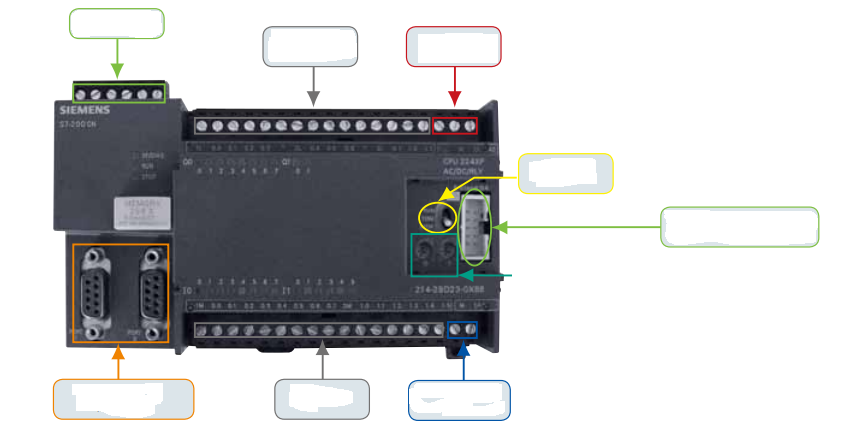
\includegraphics[angle=0,width=500pt,trim=0 0 0 0,clip]{picture/200plc.png}%答案需要替换下图片
		\tupian{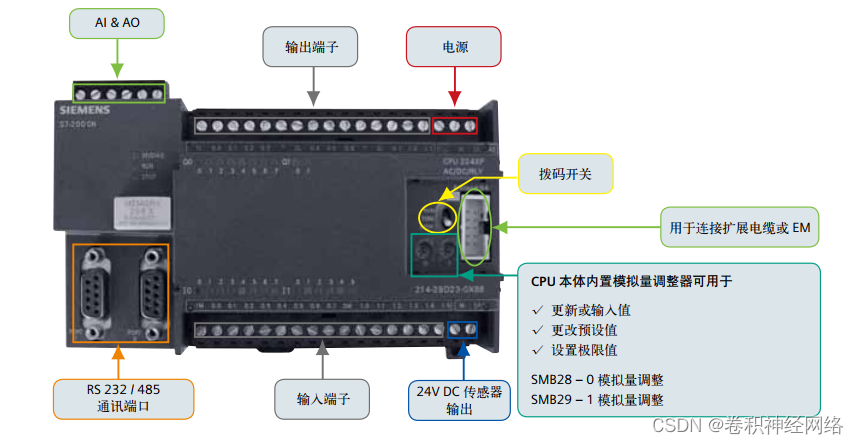
\includegraphics[angle=0,width=500pt,trim=0 0 0 0,clip]{picture/200plc_da.png}}{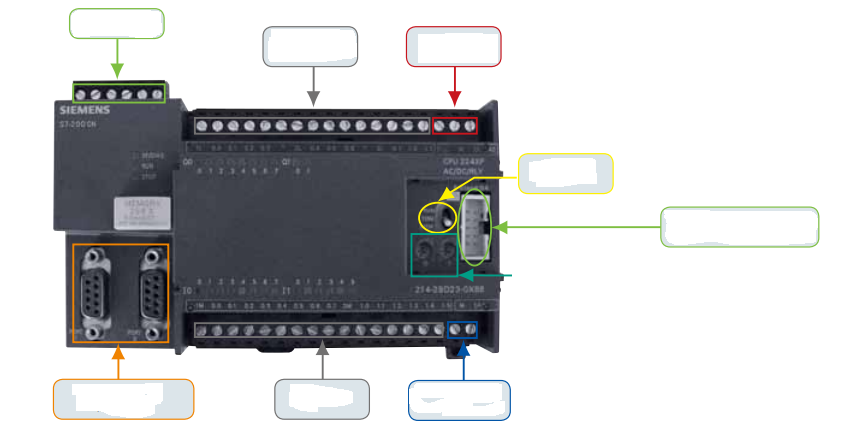
\includegraphics[angle=0,width=500pt,trim=0 0 0 0,clip]{picture/200plc.png}}
					%\includegraphics[angle=0,width=500pt,trim=0 0 0 0,clip]{picture/200plcda.png}%带答案图片
				\item 下图是一个简单的PLC线圈自锁梯形图,可以发现其逻辑关系与电路原理及其相似,画出电路图\fenzhi{14}
					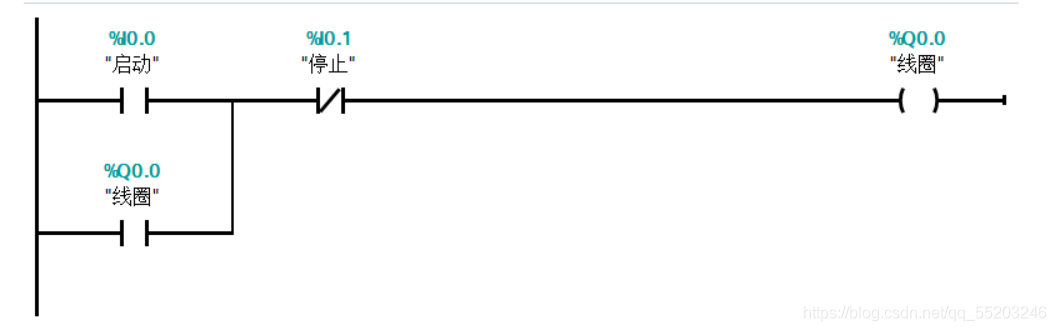
\includegraphics[angle=0,width=500pt,trim=0 0 0 0,clip]{picture/plclogic.png}    
					\wdt[5]{答:\\
						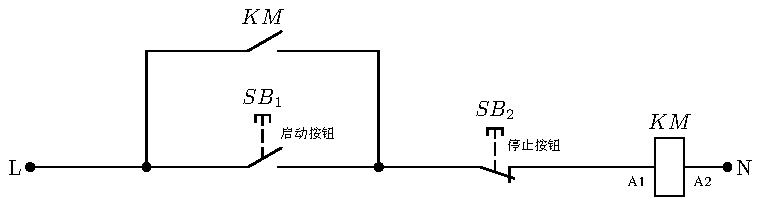
\includegraphics[angle=0,width=500pt,trim=0 0 0 0,clip]{picture/relay.pdf}    
					}
			\end{enumerate}
		\section{\htt{30}}
			\begin{enumerate}
				\setcounter{enumi}{11}
				\item 用PLC梯形图画出三取二逻辑图,输入为I0.0、I0.1、I0.2,输出为Q0.0。\fenzhi{10}
					\wdt[5]{答:\\
						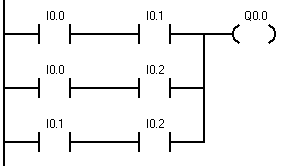
\includegraphics[angle=0,width=200pt,trim=0 0 0 0,clip]{picture/sanquerplc.png} 
					}
				\item 我厂净烟气二氧化硫分析仪模拟量输出为双量程自动切换输出,配合模拟量量程切换有一个高低量程开关量输出,即仪表显示小于50时模拟量通道量程为0-50,高低量程开关量输出为0,大于50时模拟量通道量程自动切为0-200,高低量程开关量输出变为1,而DCS系统AI通道没有切换功能,在DCS系统如何正常显示分析仪二氧化硫数据\fenzhi{20}
					\wdt[5]{答:
原理:分析仪高低量程切换过程中对应高低量程开关量由0变为1的同时模拟量输出通道毫安值缩小了$(200/50)$倍,在DCS系统逻辑内用采集到的高低量程开关量对应还原通道采集到的模拟量。\\
1.DCS量程设定:0-50(6分);\\
2.实现方法:在逻辑内通过高低量程开关量实现选择(6分);\\
3.关键点:高量程是低量程的4倍,同样数据时对应毫安信号变化为1/4倍。(6分)
					}

\end{enumerate}
		\ifx \allfiles \undefined
\end{document}
\fi
